% Options for packages loaded elsewhere
\PassOptionsToPackage{unicode}{hyperref}
\PassOptionsToPackage{hyphens}{url}
\PassOptionsToPackage{dvipsnames,svgnames,x11names}{xcolor}
%
\documentclass[
  10pt,
  presentation]{beamer}

\usepackage{amsmath,amssymb}
\usepackage{iftex}
\ifPDFTeX
  \usepackage[T1]{fontenc}
  \usepackage[utf8]{inputenc}
  \usepackage{textcomp} % provide euro and other symbols
\else % if luatex or xetex
  \usepackage{unicode-math}
  \defaultfontfeatures{Scale=MatchLowercase}
  \defaultfontfeatures[\rmfamily]{Ligatures=TeX,Scale=1}
\fi
\usepackage{lmodern}
\ifPDFTeX\else  
    % xetex/luatex font selection
\fi
% Use upquote if available, for straight quotes in verbatim environments
\IfFileExists{upquote.sty}{\usepackage{upquote}}{}
\IfFileExists{microtype.sty}{% use microtype if available
  \usepackage[]{microtype}
  \UseMicrotypeSet[protrusion]{basicmath} % disable protrusion for tt fonts
}{}
\makeatletter
\@ifundefined{KOMAClassName}{% if non-KOMA class
  \IfFileExists{parskip.sty}{%
    \usepackage{parskip}
  }{% else
    \setlength{\parindent}{0pt}
    \setlength{\parskip}{6pt plus 2pt minus 1pt}}
}{% if KOMA class
  \KOMAoptions{parskip=half}}
\makeatother
\usepackage{xcolor}
\setlength{\emergencystretch}{3em} % prevent overfull lines
\setcounter{secnumdepth}{-\maxdimen} % remove section numbering
% Make \paragraph and \subparagraph free-standing
\makeatletter
\ifx\paragraph\undefined\else
  \let\oldparagraph\paragraph
  \renewcommand{\paragraph}{
    \@ifstar
      \xxxParagraphStar
      \xxxParagraphNoStar
  }
  \newcommand{\xxxParagraphStar}[1]{\oldparagraph*{#1}\mbox{}}
  \newcommand{\xxxParagraphNoStar}[1]{\oldparagraph{#1}\mbox{}}
\fi
\ifx\subparagraph\undefined\else
  \let\oldsubparagraph\subparagraph
  \renewcommand{\subparagraph}{
    \@ifstar
      \xxxSubParagraphStar
      \xxxSubParagraphNoStar
  }
  \newcommand{\xxxSubParagraphStar}[1]{\oldsubparagraph*{#1}\mbox{}}
  \newcommand{\xxxSubParagraphNoStar}[1]{\oldsubparagraph{#1}\mbox{}}
\fi
\makeatother

\usepackage{color}
\usepackage{fancyvrb}
\newcommand{\VerbBar}{|}
\newcommand{\VERB}{\Verb[commandchars=\\\{\}]}
\DefineVerbatimEnvironment{Highlighting}{Verbatim}{commandchars=\\\{\}}
% Add ',fontsize=\small' for more characters per line
\usepackage{framed}
\definecolor{shadecolor}{RGB}{241,243,245}
\newenvironment{Shaded}{\begin{snugshade}}{\end{snugshade}}
\newcommand{\AlertTok}[1]{\textcolor[rgb]{0.68,0.00,0.00}{#1}}
\newcommand{\AnnotationTok}[1]{\textcolor[rgb]{0.37,0.37,0.37}{#1}}
\newcommand{\AttributeTok}[1]{\textcolor[rgb]{0.40,0.45,0.13}{#1}}
\newcommand{\BaseNTok}[1]{\textcolor[rgb]{0.68,0.00,0.00}{#1}}
\newcommand{\BuiltInTok}[1]{\textcolor[rgb]{0.00,0.23,0.31}{#1}}
\newcommand{\CharTok}[1]{\textcolor[rgb]{0.13,0.47,0.30}{#1}}
\newcommand{\CommentTok}[1]{\textcolor[rgb]{0.37,0.37,0.37}{#1}}
\newcommand{\CommentVarTok}[1]{\textcolor[rgb]{0.37,0.37,0.37}{\textit{#1}}}
\newcommand{\ConstantTok}[1]{\textcolor[rgb]{0.56,0.35,0.01}{#1}}
\newcommand{\ControlFlowTok}[1]{\textcolor[rgb]{0.00,0.23,0.31}{\textbf{#1}}}
\newcommand{\DataTypeTok}[1]{\textcolor[rgb]{0.68,0.00,0.00}{#1}}
\newcommand{\DecValTok}[1]{\textcolor[rgb]{0.68,0.00,0.00}{#1}}
\newcommand{\DocumentationTok}[1]{\textcolor[rgb]{0.37,0.37,0.37}{\textit{#1}}}
\newcommand{\ErrorTok}[1]{\textcolor[rgb]{0.68,0.00,0.00}{#1}}
\newcommand{\ExtensionTok}[1]{\textcolor[rgb]{0.00,0.23,0.31}{#1}}
\newcommand{\FloatTok}[1]{\textcolor[rgb]{0.68,0.00,0.00}{#1}}
\newcommand{\FunctionTok}[1]{\textcolor[rgb]{0.28,0.35,0.67}{#1}}
\newcommand{\ImportTok}[1]{\textcolor[rgb]{0.00,0.46,0.62}{#1}}
\newcommand{\InformationTok}[1]{\textcolor[rgb]{0.37,0.37,0.37}{#1}}
\newcommand{\KeywordTok}[1]{\textcolor[rgb]{0.00,0.23,0.31}{\textbf{#1}}}
\newcommand{\NormalTok}[1]{\textcolor[rgb]{0.00,0.23,0.31}{#1}}
\newcommand{\OperatorTok}[1]{\textcolor[rgb]{0.37,0.37,0.37}{#1}}
\newcommand{\OtherTok}[1]{\textcolor[rgb]{0.00,0.23,0.31}{#1}}
\newcommand{\PreprocessorTok}[1]{\textcolor[rgb]{0.68,0.00,0.00}{#1}}
\newcommand{\RegionMarkerTok}[1]{\textcolor[rgb]{0.00,0.23,0.31}{#1}}
\newcommand{\SpecialCharTok}[1]{\textcolor[rgb]{0.37,0.37,0.37}{#1}}
\newcommand{\SpecialStringTok}[1]{\textcolor[rgb]{0.13,0.47,0.30}{#1}}
\newcommand{\StringTok}[1]{\textcolor[rgb]{0.13,0.47,0.30}{#1}}
\newcommand{\VariableTok}[1]{\textcolor[rgb]{0.07,0.07,0.07}{#1}}
\newcommand{\VerbatimStringTok}[1]{\textcolor[rgb]{0.13,0.47,0.30}{#1}}
\newcommand{\WarningTok}[1]{\textcolor[rgb]{0.37,0.37,0.37}{\textit{#1}}}

\providecommand{\tightlist}{%
  \setlength{\itemsep}{0pt}\setlength{\parskip}{0pt}}\usepackage{longtable,booktabs,array}
\usepackage{calc} % for calculating minipage widths
% Correct order of tables after \paragraph or \subparagraph
\usepackage{etoolbox}
\makeatletter
\patchcmd\longtable{\par}{\if@noskipsec\mbox{}\fi\par}{}{}
\makeatother
% Allow footnotes in longtable head/foot
\IfFileExists{footnotehyper.sty}{\usepackage{footnotehyper}}{\usepackage{footnote}}
\makesavenoteenv{longtable}
\usepackage{graphicx}
\makeatletter
\newsavebox\pandoc@box
\newcommand*\pandocbounded[1]{% scales image to fit in text height/width
  \sbox\pandoc@box{#1}%
  \Gscale@div\@tempa{\textheight}{\dimexpr\ht\pandoc@box+\dp\pandoc@box\relax}%
  \Gscale@div\@tempb{\linewidth}{\wd\pandoc@box}%
  \ifdim\@tempb\p@<\@tempa\p@\let\@tempa\@tempb\fi% select the smaller of both
  \ifdim\@tempa\p@<\p@\scalebox{\@tempa}{\usebox\pandoc@box}%
  \else\usebox{\pandoc@box}%
  \fi%
}
% Set default figure placement to htbp
\def\fps@figure{htbp}
\makeatother
% definitions for citeproc citations
\NewDocumentCommand\citeproctext{}{}
\NewDocumentCommand\citeproc{mm}{%
  \begingroup\def\citeproctext{#2}\cite{#1}\endgroup}
\makeatletter
 % allow citations to break across lines
 \let\@cite@ofmt\@firstofone
 % avoid brackets around text for \cite:
 \def\@biblabel#1{}
 \def\@cite#1#2{{#1\if@tempswa , #2\fi}}
\makeatother
\newlength{\cslhangindent}
\setlength{\cslhangindent}{1.5em}
\newlength{\csllabelwidth}
\setlength{\csllabelwidth}{3em}
\newenvironment{CSLReferences}[2] % #1 hanging-indent, #2 entry-spacing
 {\begin{list}{}{%
  \setlength{\itemindent}{0pt}
  \setlength{\leftmargin}{0pt}
  \setlength{\parsep}{0pt}
  % turn on hanging indent if param 1 is 1
  \ifodd #1
   \setlength{\leftmargin}{\cslhangindent}
   \setlength{\itemindent}{-1\cslhangindent}
  \fi
  % set entry spacing
  \setlength{\itemsep}{#2\baselineskip}}}
 {\end{list}}
\usepackage{calc}
\newcommand{\CSLBlock}[1]{\hfill\break\parbox[t]{\linewidth}{\strut\ignorespaces#1\strut}}
\newcommand{\CSLLeftMargin}[1]{\parbox[t]{\csllabelwidth}{\strut#1\strut}}
\newcommand{\CSLRightInline}[1]{\parbox[t]{\linewidth - \csllabelwidth}{\strut#1\strut}}
\newcommand{\CSLIndent}[1]{\hspace{\cslhangindent}#1}

\makeatletter
\@ifpackageloaded{caption}{}{\usepackage{caption}}
\AtBeginDocument{%
\ifdefined\contentsname
  \renewcommand*\contentsname{Содержание}
\else
  \newcommand\contentsname{Содержание}
\fi
\ifdefined\listfigurename
  \renewcommand*\listfigurename{Список иллюстраций}
\else
  \newcommand\listfigurename{Список иллюстраций}
\fi
\ifdefined\listtablename
  \renewcommand*\listtablename{Список таблиц}
\else
  \newcommand\listtablename{Список таблиц}
\fi
\ifdefined\figurename
  \renewcommand*\figurename{Рисунок}
\else
  \newcommand\figurename{Рисунок}
\fi
\ifdefined\tablename
  \renewcommand*\tablename{Таблица}
\else
  \newcommand\tablename{Таблица}
\fi
}
\@ifpackageloaded{float}{}{\usepackage{float}}
\floatstyle{ruled}
\@ifundefined{c@chapter}{\newfloat{codelisting}{h}{lop}}{\newfloat{codelisting}{h}{lop}[chapter]}
\floatname{codelisting}{Список}
\newcommand*\listoflistings{\listof{codelisting}{Листинги}}
\makeatother
\makeatletter
\makeatother
\makeatletter
\@ifpackageloaded{caption}{}{\usepackage{caption}}
\@ifpackageloaded{subcaption}{}{\usepackage{subcaption}}
\makeatother

\ifLuaTeX
\usepackage[bidi=basic]{babel}
\else
\usepackage[bidi=default]{babel}
\fi
\babelprovide[main,import]{russian}
\babelprovide[import]{english}
% get rid of language-specific shorthands (see #6817):
\let\LanguageShortHands\languageshorthands
\def\languageshorthands#1{}
\usepackage{bookmark}

\IfFileExists{xurl.sty}{\usepackage{xurl}}{} % add URL line breaks if available
\urlstyle{same} % disable monospaced font for URLs
\hypersetup{
  pdftitle={Презентация по лабораторной работе №3},
  pdfauthor={Черная София Витальевна},
  pdflang={ru},
  colorlinks=true,
  linkcolor={blue},
  filecolor={Maroon},
  citecolor={Blue},
  urlcolor={Blue},
  pdfcreator={LaTeX via pandoc}}


\title{Презентация по лабораторной работе №3}
\usepackage{etoolbox}
\makeatletter
\providecommand{\subtitle}[1]{% add subtitle to \maketitle
  \apptocmd{\@title}{\par {\large #1 \par}}{}{}
}
\makeatother
\subtitle{Агентное моделирование. Модель Daisyworld}
\author{Черная София Витальевна}
\date{2026-03-21}

\begin{document}
\maketitle


\section{Информация}\label{ux438ux43dux444ux43eux440ux43cux430ux446ux438ux44f}

\subsection{Докладчик}\label{ux434ux43eux43aux43bux430ux434ux447ux438ux43a}

\begin{itemize}
\tightlist
\item
  Черная София Витальевна
\item
  Студентка
\item
  Российский университет дружбы народов им. Патриса Лумумбы
\item
  {[}1132236043@rudn.ru{]}
\end{itemize}

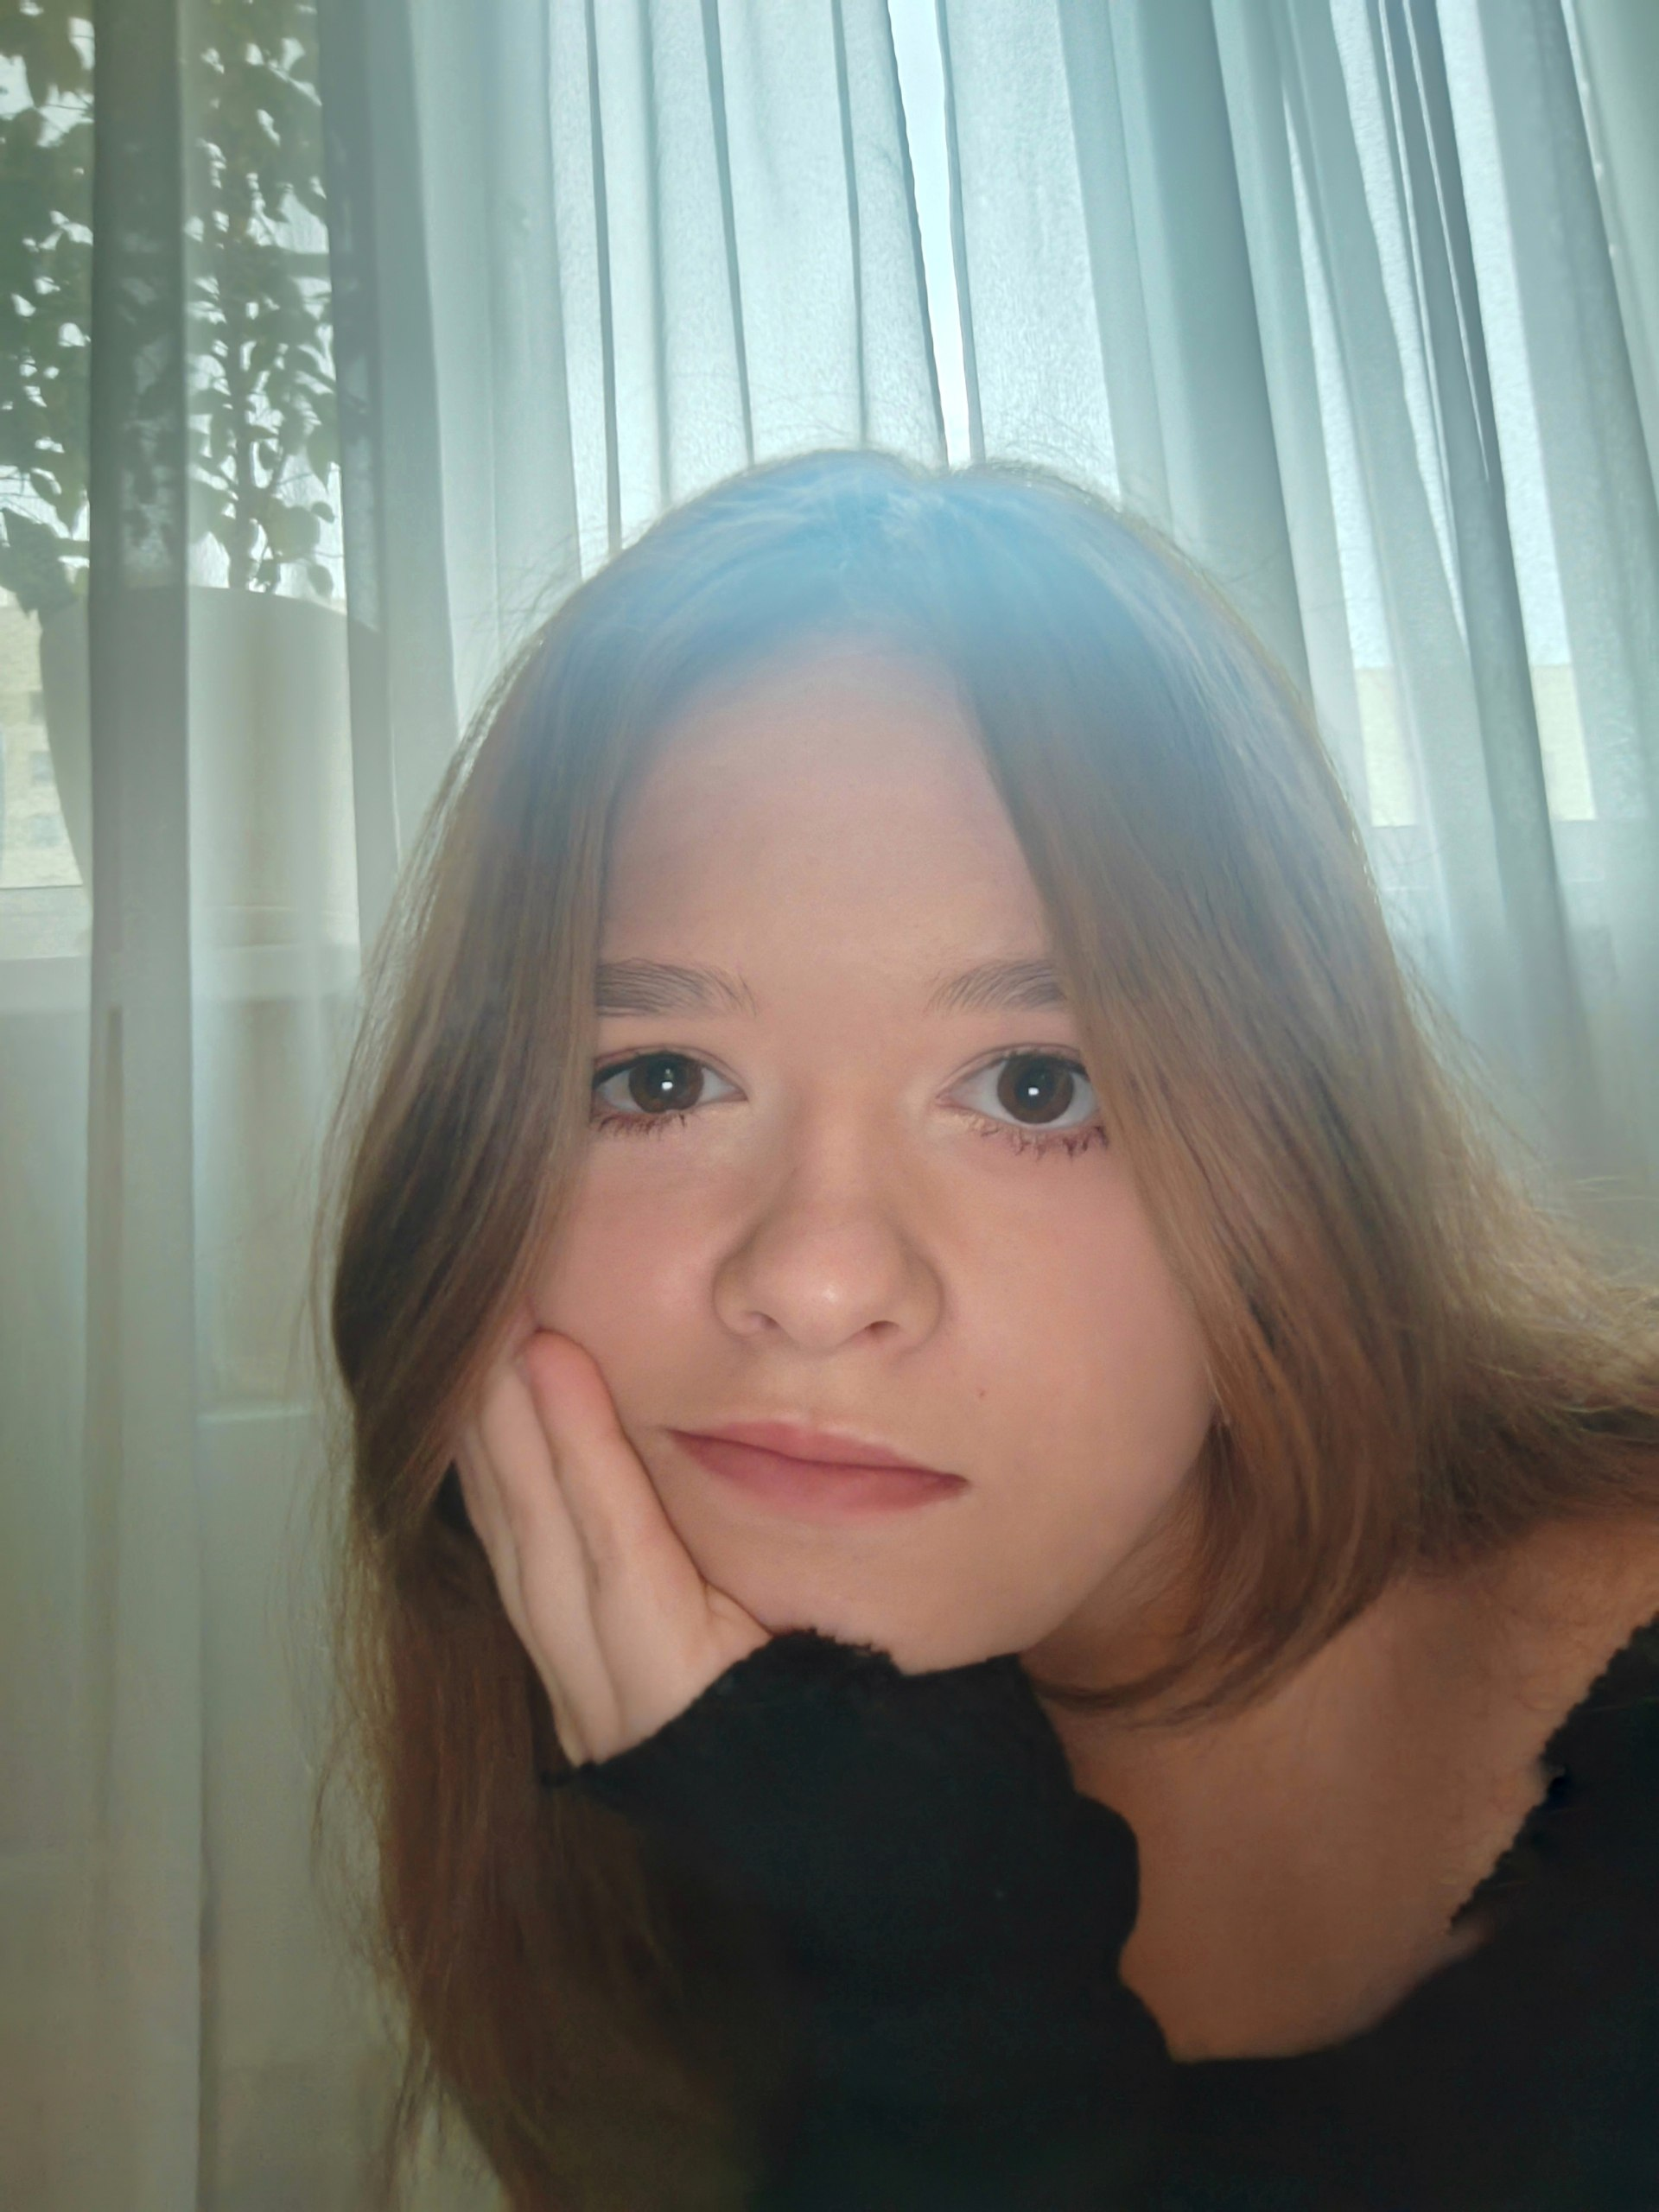
\includegraphics[width=0.8\linewidth,height=\textheight,keepaspectratio]{image/photo.jpg}

\section{Теоретическое
введение}\label{ux442ux435ux43eux440ux435ux442ux438ux447ux435ux441ux43aux43eux435-ux432ux432ux435ux434ux435ux43dux438ux435}

\subsection{Агентный
подход}\label{ux430ux433ux435ux43dux442ux43dux44bux439-ux43fux43eux434ux445ux43eux434}

Агентный подход к имитационному моделированию (Agent-Based Modeling,
ABM) --- это метод исследования сложных систем, в котором поведение
системы возникает из взаимодействия множества автономных сущностей,
называемых \textbf{агентами}.

\textbf{Ключевые компоненты:} - \textbf{Агенты} --- активные сущности с
правилами поведения - \textbf{Среда} --- пространство существования
агентов - \textbf{Взаимодействия} --- правила влияния агентов друг на
друга и среду

\subsection{Модель
Daisyworld}\label{ux43cux43eux434ux435ux43bux44c-daisyworld}

Модель была разработана Джеймсом Лавлоком для демонстрации
\textbf{гипотезы Геи} --- идеи о том, что планета является
саморегулирующейся системой.

\begin{itemize}
\tightlist
\item
  \textbf{Белые маргаритки} --- высокое альбедо (0.75) →
  \textbf{охлаждают} планету
\item
  \textbf{Черные маргаритки} --- низкое альбедо (0.25) →
  \textbf{нагревают} планету
\end{itemize}

\textbf{Механизм обратной связи:} - Слишком жарко → размножаются белые
маргаритки → охлаждение - Слишком холодно → размножаются черные
маргаритки → нагрев

\section{Выполнение лабораторной
работы}\label{ux432ux44bux43fux43eux43bux43dux435ux43dux438ux435-ux43bux430ux431ux43eux440ux430ux442ux43eux440ux43dux43eux439-ux440ux430ux431ux43eux442ux44b}

\subsection{Создание
модели}\label{ux441ux43eux437ux434ux430ux43dux438ux435-ux43cux43eux434ux435ux43bux438}

Создаю файл \texttt{src/daisyworld.jl} с определением агента-маргаритки
(рис.~\ref{fig-001})

\begin{figure}

\centering{


\includegraphics[width=0.7\linewidth,height=\textheight,keepaspectratio]{image/3.png}

}

\caption{\label{fig-001}Создание файла модели}

\end{figure}%

\subsection{Код
модели}\label{ux43aux43eux434-ux43cux43eux434ux435ux43bux438}

Основные компоненты модели:

\begin{Shaded}
\begin{Highlighting}[]
\PreprocessorTok{@agent} \KeywordTok{struct} \FunctionTok{Daisy}\NormalTok{(NoSpaceAgent)}
\NormalTok{    breed}\OperatorTok{::}\DataTypeTok{Symbol   }\CommentTok{\# :black или :white}
\NormalTok{    age}\OperatorTok{::}\DataTypeTok{Int        }\CommentTok{\# возраст маргаритки}
\NormalTok{    albedo}\OperatorTok{::}\DataTypeTok{Float64 }\CommentTok{\# альбедо (0.25 или 0.75)}
\KeywordTok{end}
\end{Highlighting}
\end{Shaded}

Функции: - \texttt{local\_temperature()} --- расчет локальной
температуры с учетом альбедо - \texttt{diffuse\_temperature()} ---
диффузия тепла между соседними клетками -
\texttt{reproduction\_probability()} --- вероятность размножения в
зависимости от температуры

\subsection{Визуализация
модели}\label{ux432ux438ux437ux443ux430ux43bux438ux437ux430ux446ux438ux44f-ux43cux43eux434ux435ux43bux438}

Создаю скрипт визуализации, который сохраняет три снимка состояния мира
(рис.~\ref{fig-002})

\begin{figure}

\centering{


\includegraphics[width=0.7\linewidth,height=\textheight,keepaspectratio]{image/6.png}

}

\caption{\label{fig-002}Код скрипта визуализации}

\end{figure}%

\subsection{Результаты
визуализации}\label{ux440ux435ux437ux443ux43bux44cux442ux430ux442ux44b-ux432ux438ux437ux443ux430ux43bux438ux437ux430ux446ux438ux438}

\textbf{Начальное состояние} (шаг 0) (рис.~\ref{fig-003})

\begin{figure}

\centering{


\includegraphics[width=0.7\linewidth,height=\textheight,keepaspectratio]{image/11.png}

}

\caption{\label{fig-003}Начальное состояние}

\end{figure}%

Черные и белые маргаритки распределены равномерно

\subsection{Результаты
визуализации}\label{ux440ux435ux437ux443ux43bux44cux442ux430ux442ux44b-ux432ux438ux437ux443ux430ux43bux438ux437ux430ux446ux438ux438-1}

\textbf{Состояние через 5 шагов} (рис.~\ref{fig-004})

\begin{figure}

\centering{


\includegraphics[width=0.7\linewidth,height=\textheight,keepaspectratio]{image/12.png}

}

\caption{\label{fig-004}5 шагов}

\end{figure}%

Активное размножение, занятие свободных клеток

\subsection{Результаты
визуализации}\label{ux440ux435ux437ux443ux43bux44cux442ux430ux442ux44b-ux432ux438ux437ux443ux430ux43bux438ux437ux430ux446ux438ux438-2}

\textbf{Состояние через 40 шагов} (рис.~\ref{fig-005})

\begin{figure}

\centering{


\includegraphics[width=0.7\linewidth,height=\textheight,keepaspectratio]{image/13.png}

}

\caption{\label{fig-005}40 шагов}

\end{figure}%

Устойчивое состояние, все клетки заняты

\section{Анализ динамики
популяции}\label{ux430ux43dux430ux43bux438ux437-ux434ux438ux43dux430ux43cux438ux43aux438-ux43fux43eux43fux443ux43bux44fux446ux438ux438}

\subsection{Динамика
численности}\label{ux434ux438ux43dux430ux43cux438ux43aux430-ux447ux438ux441ux43bux435ux43dux43dux43eux441ux442ux438}

Создаю скрипт \texttt{daisyworld-count.jl} для отслеживания численности
(рис.~\ref{fig-006})

\begin{figure}

\centering{


\includegraphics[width=0.7\linewidth,height=\textheight,keepaspectratio]{image/26.png}

}

\caption{\label{fig-006}Код скрипта}

\end{figure}%

\subsection{График динамики
численности}\label{ux433ux440ux430ux444ux438ux43a-ux434ux438ux43dux430ux43cux438ux43aux438-ux447ux438ux441ux43bux435ux43dux43dux43eux441ux442ux438}

\begin{figure}

\centering{


\includegraphics[width=0.8\linewidth,height=\textheight,keepaspectratio]{image/27.png}

}

\caption{\label{fig-007}Динамика численности черных и белых маргариток}

\end{figure}%

\textbf{Выводы:} - Черные маргаритки доминируют на протяжении всей
симуляции - Наблюдаются колебания численности - Система достигает
динамического равновесия

\section{Исследование при изменяющейся
светимости}\label{ux438ux441ux441ux43bux435ux434ux43eux432ux430ux43dux438ux435-ux43fux440ux438-ux438ux437ux43cux435ux43dux44fux44eux449ux435ux439ux441ux44f-ux441ux432ux435ux442ux438ux43cux43eux441ux442ux438}

\subsection{Сценарий
:ramp}\label{ux441ux446ux435ux43dux430ux440ux438ux439-ramp}

Создаю скрипт \texttt{daisyworld-luminosity.jl} для анализа при
изменяющейся солнечной активности (рис.~\ref{fig-008})

\begin{figure}

\centering{


\includegraphics[width=0.7\linewidth,height=\textheight,keepaspectratio]{image/32.png}

}

\caption{\label{fig-008}Код скрипта}

\end{figure}%

\subsection{Комплексный
график}\label{ux43aux43eux43cux43fux43bux435ux43aux441ux43dux44bux439-ux433ux440ux430ux444ux438ux43a}

\begin{figure}

\centering{

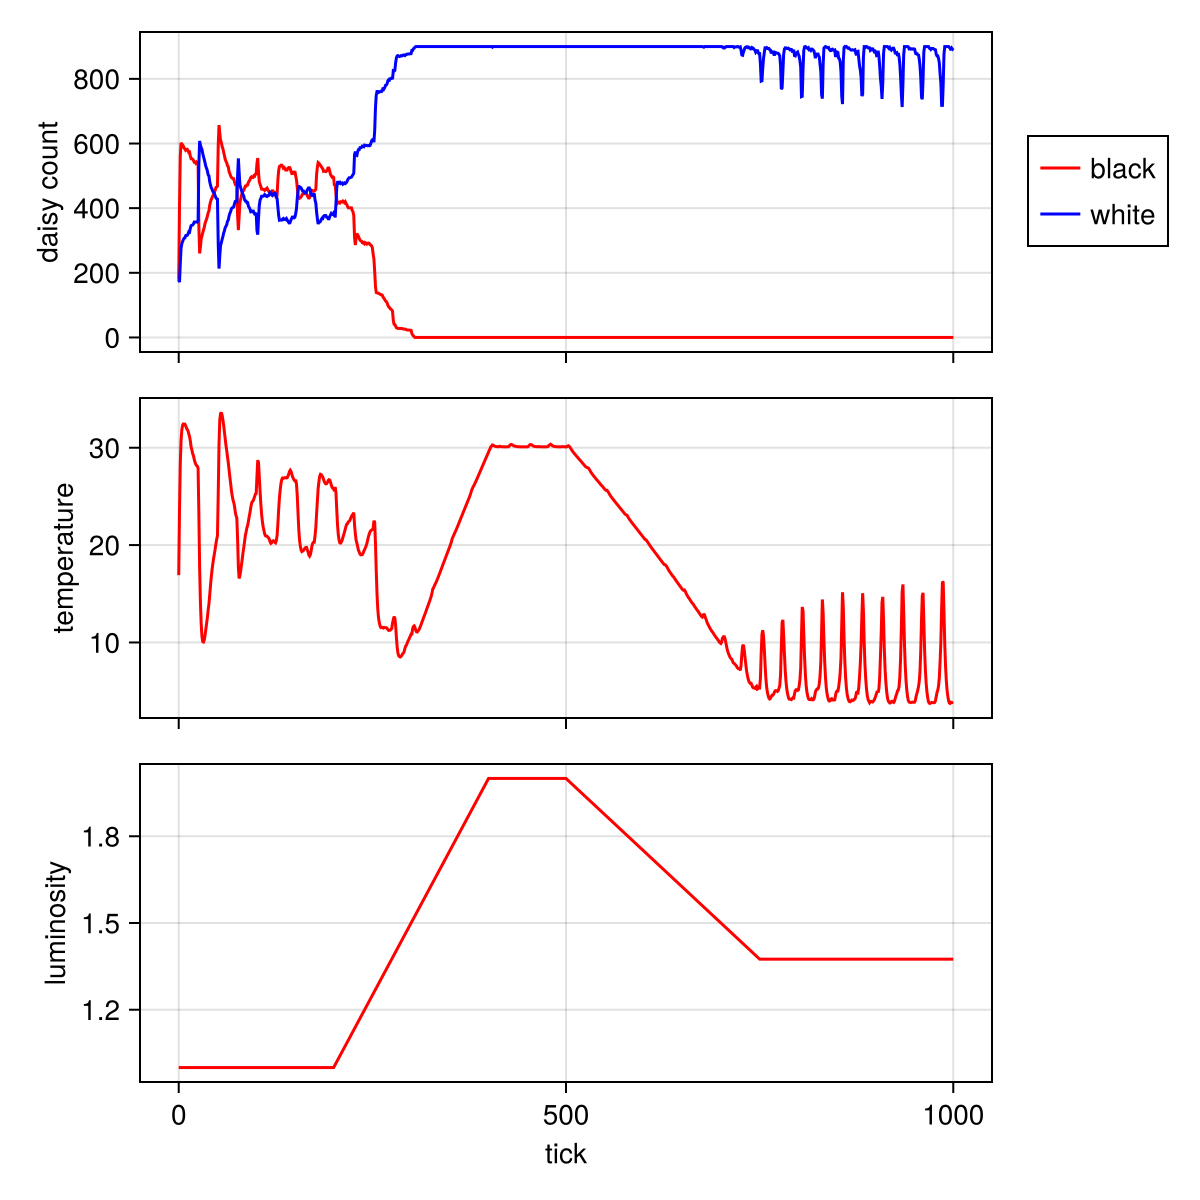
\includegraphics[width=0.8\linewidth,height=\textheight,keepaspectratio]{image/daisy_luminosity.png}

}

\caption{\label{fig-009}Динамика популяций, температуры и светимости}

\end{figure}%

\textbf{Выводы:} - Маргаритки компенсируют изменение внешней светимости
- Температура остается стабильной в широком диапазоне - Демонстрация
механизма отрицательной обратной связи

\section{Параметрическое
исследование}\label{ux43fux430ux440ux430ux43cux435ux442ux440ux438ux447ux435ux441ux43aux43eux435-ux438ux441ux441ux43bux435ux434ux43eux432ux430ux43dux438ux435}

\subsection{Пространственное
распределение}\label{ux43fux440ux43eux441ux442ux440ux430ux43dux441ux442ux432ux435ux43dux43dux43eux435-ux440ux430ux441ux43fux440ux435ux434ux435ux43bux435ux43dux438ux435}

\textbf{Серия 1:} max\_age=25, init\_white=0.2

\begin{longtable}[]{@{}
  >{\centering\arraybackslash}p{(\linewidth - 4\tabcolsep) * \real{0.4038}}
  >{\centering\arraybackslash}p{(\linewidth - 4\tabcolsep) * \real{0.2885}}
  >{\centering\arraybackslash}p{(\linewidth - 4\tabcolsep) * \real{0.3077}}@{}}
\toprule\noalign{}
\begin{minipage}[b]{\linewidth}\centering
Начальное состояние
\end{minipage} & \begin{minipage}[b]{\linewidth}\centering
Через 5 шагов
\end{minipage} & \begin{minipage}[b]{\linewidth}\centering
Через 40 шагов
\end{minipage} \\
\midrule\noalign{}
\endhead
\bottomrule\noalign{}
\endlastfoot

\includegraphics[width=1\linewidth,height=\textheight,keepaspectratio]{image/40.png}
&

\includegraphics[width=1\linewidth,height=\textheight,keepaspectratio]{image/41.png}
&

\includegraphics[width=1\linewidth,height=\textheight,keepaspectratio]{image/42.png} \\
\end{longtable}

Преобладание черных маргариток

\subsection{Пространственное
распределение}\label{ux43fux440ux43eux441ux442ux440ux430ux43dux441ux442ux432ux435ux43dux43dux43eux435-ux440ux430ux441ux43fux440ux435ux434ux435ux43bux435ux43dux438ux435-1}

\textbf{Серия 2:} max\_age=40, init\_white=0.2

\begin{longtable}[]{@{}
  >{\centering\arraybackslash}p{(\linewidth - 4\tabcolsep) * \real{0.4038}}
  >{\centering\arraybackslash}p{(\linewidth - 4\tabcolsep) * \real{0.2885}}
  >{\centering\arraybackslash}p{(\linewidth - 4\tabcolsep) * \real{0.3077}}@{}}
\toprule\noalign{}
\begin{minipage}[b]{\linewidth}\centering
Начальное состояние
\end{minipage} & \begin{minipage}[b]{\linewidth}\centering
Через 5 шагов
\end{minipage} & \begin{minipage}[b]{\linewidth}\centering
Через 40 шагов
\end{minipage} \\
\midrule\noalign{}
\endhead
\bottomrule\noalign{}
\endlastfoot

\includegraphics[width=1\linewidth,height=\textheight,keepaspectratio]{image/43.png}
&

\includegraphics[width=1\linewidth,height=\textheight,keepaspectratio]{image/44.png}
&

\includegraphics[width=1\linewidth,height=\textheight,keepaspectratio]{image/45.png} \\
\end{longtable}

Более высокая численность, больше белых

\subsection{Пространственное
распределение}\label{ux43fux440ux43eux441ux442ux440ux430ux43dux441ux442ux432ux435ux43dux43dux43eux435-ux440ux430ux441ux43fux440ux435ux434ux435ux43bux435ux43dux438ux435-2}

\textbf{Серия 3:} max\_age=25, init\_white=0.8

\begin{longtable}[]{@{}
  >{\centering\arraybackslash}p{(\linewidth - 4\tabcolsep) * \real{0.4038}}
  >{\centering\arraybackslash}p{(\linewidth - 4\tabcolsep) * \real{0.2885}}
  >{\centering\arraybackslash}p{(\linewidth - 4\tabcolsep) * \real{0.3077}}@{}}
\toprule\noalign{}
\begin{minipage}[b]{\linewidth}\centering
Начальное состояние
\end{minipage} & \begin{minipage}[b]{\linewidth}\centering
Через 5 шагов
\end{minipage} & \begin{minipage}[b]{\linewidth}\centering
Через 40 шагов
\end{minipage} \\
\midrule\noalign{}
\endhead
\bottomrule\noalign{}
\endlastfoot

\includegraphics[width=1\linewidth,height=\textheight,keepaspectratio]{image/46.png}
&

\includegraphics[width=1\linewidth,height=\textheight,keepaspectratio]{image/47.png}
&

\includegraphics[width=1\linewidth,height=\textheight,keepaspectratio]{image/48.png} \\
\end{longtable}

Начальное преобладание белых, затем черные вытесняют

\subsection{Пространственное
распределение}\label{ux43fux440ux43eux441ux442ux440ux430ux43dux441ux442ux432ux435ux43dux43dux43eux435-ux440ux430ux441ux43fux440ux435ux434ux435ux43bux435ux43dux438ux435-3}

\textbf{Серия 4:} max\_age=40, init\_white=0.8

\begin{longtable}[]{@{}
  >{\centering\arraybackslash}p{(\linewidth - 4\tabcolsep) * \real{0.4038}}
  >{\centering\arraybackslash}p{(\linewidth - 4\tabcolsep) * \real{0.2885}}
  >{\centering\arraybackslash}p{(\linewidth - 4\tabcolsep) * \real{0.3077}}@{}}
\toprule\noalign{}
\begin{minipage}[b]{\linewidth}\centering
Начальное состояние
\end{minipage} & \begin{minipage}[b]{\linewidth}\centering
Через 5 шагов
\end{minipage} & \begin{minipage}[b]{\linewidth}\centering
Через 40 шагов
\end{minipage} \\
\midrule\noalign{}
\endhead
\bottomrule\noalign{}
\endlastfoot

\includegraphics[width=1\linewidth,height=\textheight,keepaspectratio]{image/49.png}
&

\includegraphics[width=1\linewidth,height=\textheight,keepaspectratio]{image/50.png}
&

\includegraphics[width=1\linewidth,height=\textheight,keepaspectratio]{image/51.png} \\
\end{longtable}

Черных становится больше, чем белых

\section{Динамика численности (параметрическое
исследование)}\label{ux434ux438ux43dux430ux43cux438ux43aux430-ux447ux438ux441ux43bux435ux43dux43dux43eux441ux442ux438-ux43fux430ux440ux430ux43cux435ux442ux440ux438ux447ux435ux441ux43aux43eux435-ux438ux441ux441ux43bux435ux434ux43eux432ux430ux43dux438ux435}

\subsection{Графики
динамики}\label{ux433ux440ux430ux444ux438ux43aux438-ux434ux438ux43dux430ux43cux438ux43aux438}

\begin{longtable}[]{@{}cc@{}}
\toprule\noalign{}
max\_age=25, init\_white=0.2 & max\_age=40, init\_white=0.2 \\
\midrule\noalign{}
\endhead
\bottomrule\noalign{}
\endlastfoot

\includegraphics[width=1\linewidth,height=\textheight,keepaspectratio]{image/59.png}
&
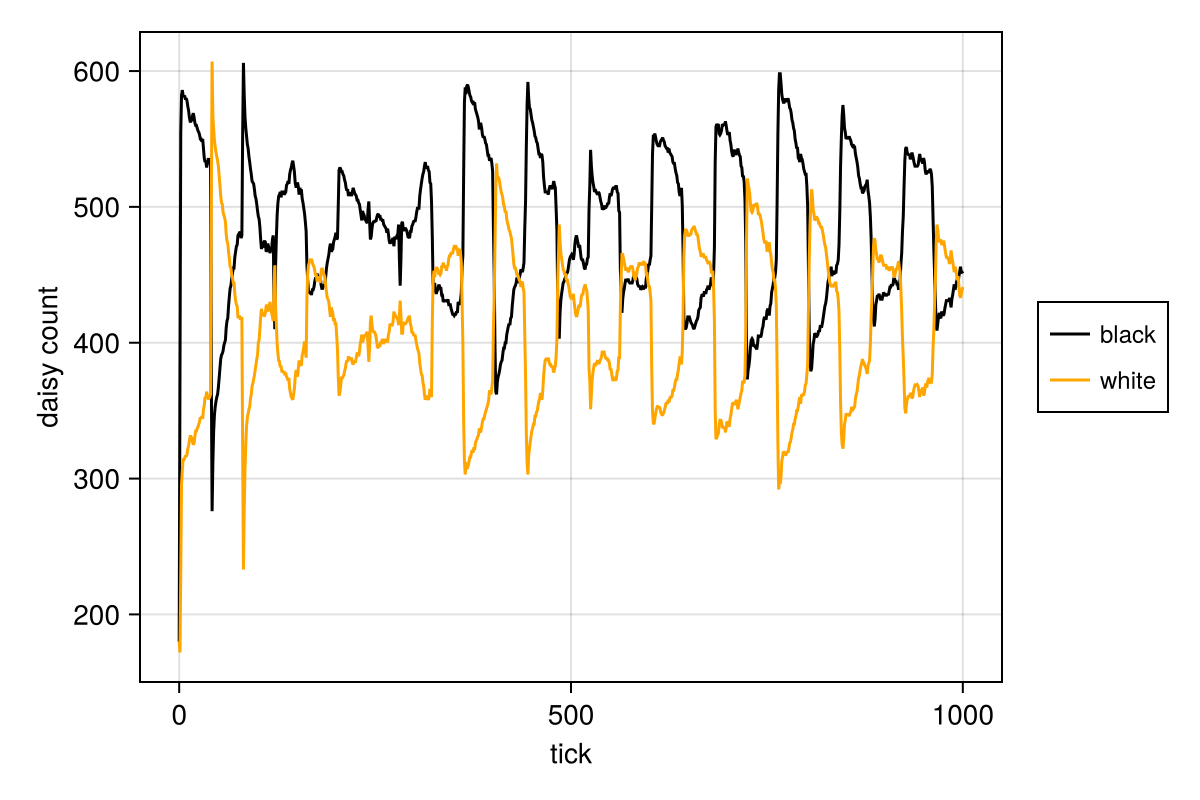
\includegraphics[width=1\linewidth,height=\textheight,keepaspectratio]{image/60.png} \\
Черные доминируют & Более сильные колебания \\
\end{longtable}

\subsection{Графики
динамики}\label{ux433ux440ux430ux444ux438ux43aux438-ux434ux438ux43dux430ux43cux438ux43aux438-1}

\begin{longtable}[]{@{}cc@{}}
\toprule\noalign{}
max\_age=25, init\_white=0.8 & max\_age=40, init\_white=0.8 \\
\midrule\noalign{}
\endhead
\bottomrule\noalign{}
\endlastfoot
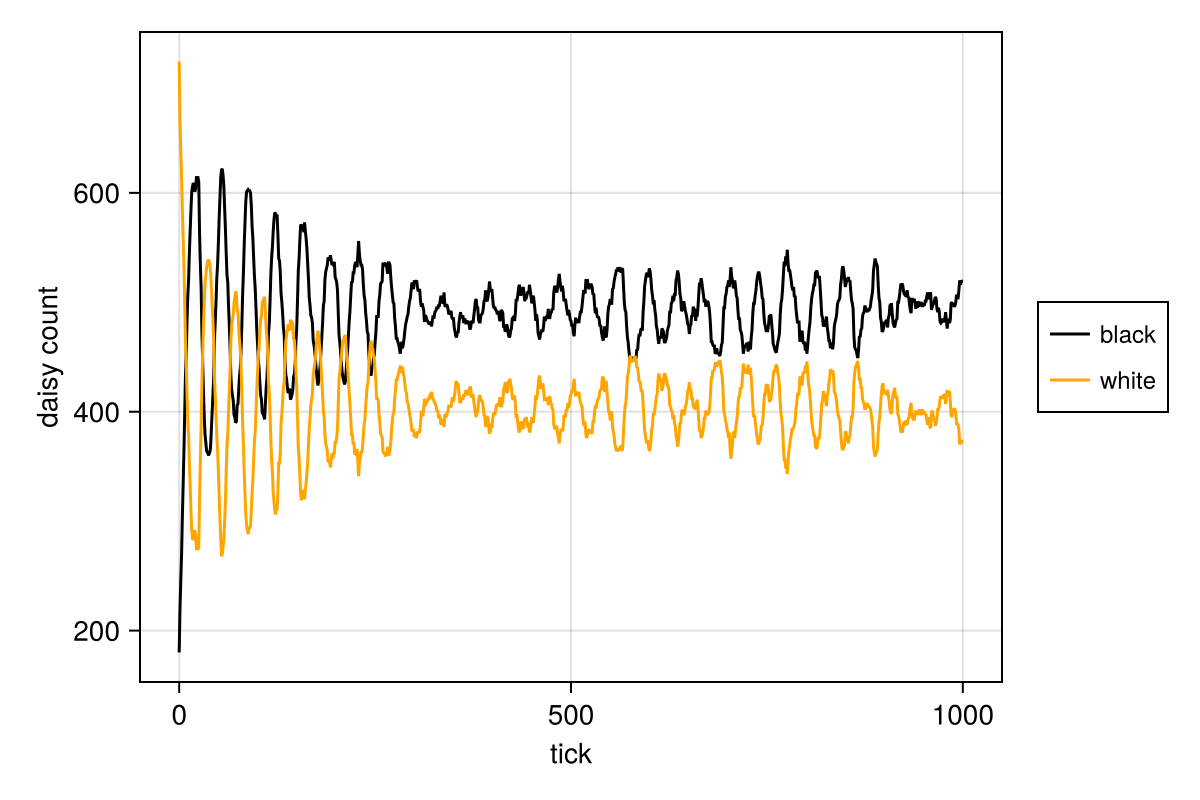
\includegraphics[width=1\linewidth,height=\textheight,keepaspectratio]{image/61.png}
&
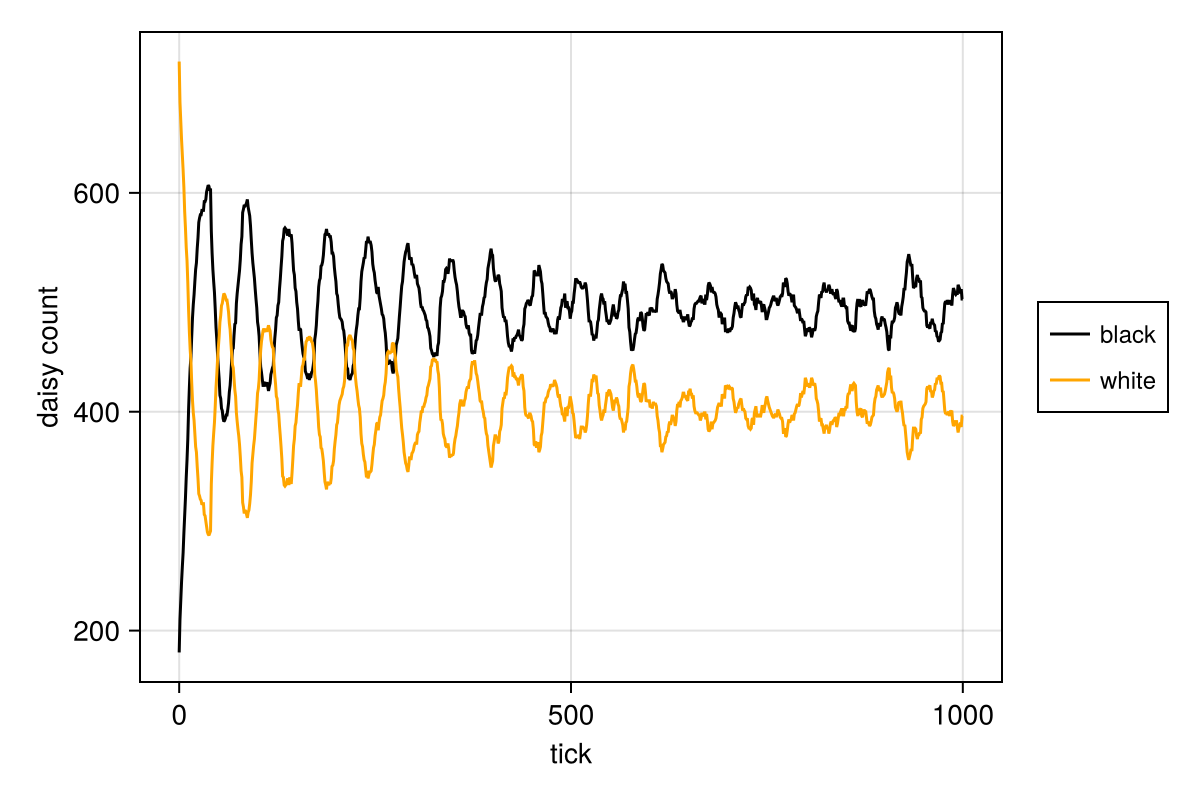
\includegraphics[width=1\linewidth,height=\textheight,keepaspectratio]{image/62.png} \\
Преобладание черных & Интервалы между колебаниями больше \\
\end{longtable}

\section{Динамика при изменяющейся светимости (параметрическое
исследование)}\label{ux434ux438ux43dux430ux43cux438ux43aux430-ux43fux440ux438-ux438ux437ux43cux435ux43dux44fux44eux449ux435ux439ux441ux44f-ux441ux432ux435ux442ux438ux43cux43eux441ux442ux438-ux43fux430ux440ux430ux43cux435ux442ux440ux438ux447ux435ux441ux43aux43eux435-ux438ux441ux441ux43bux435ux434ux43eux432ux430ux43dux438ux435}

\subsection{Комплексные
графики}\label{ux43aux43eux43cux43fux43bux435ux43aux441ux43dux44bux435-ux433ux440ux430ux444ux438ux43aux438}

\begin{longtable}[]{@{}cc@{}}
\toprule\noalign{}
max\_age=25, init\_white=0.2 & max\_age=40, init\_white=0.2 \\
\midrule\noalign{}
\endhead
\bottomrule\noalign{}
\endlastfoot
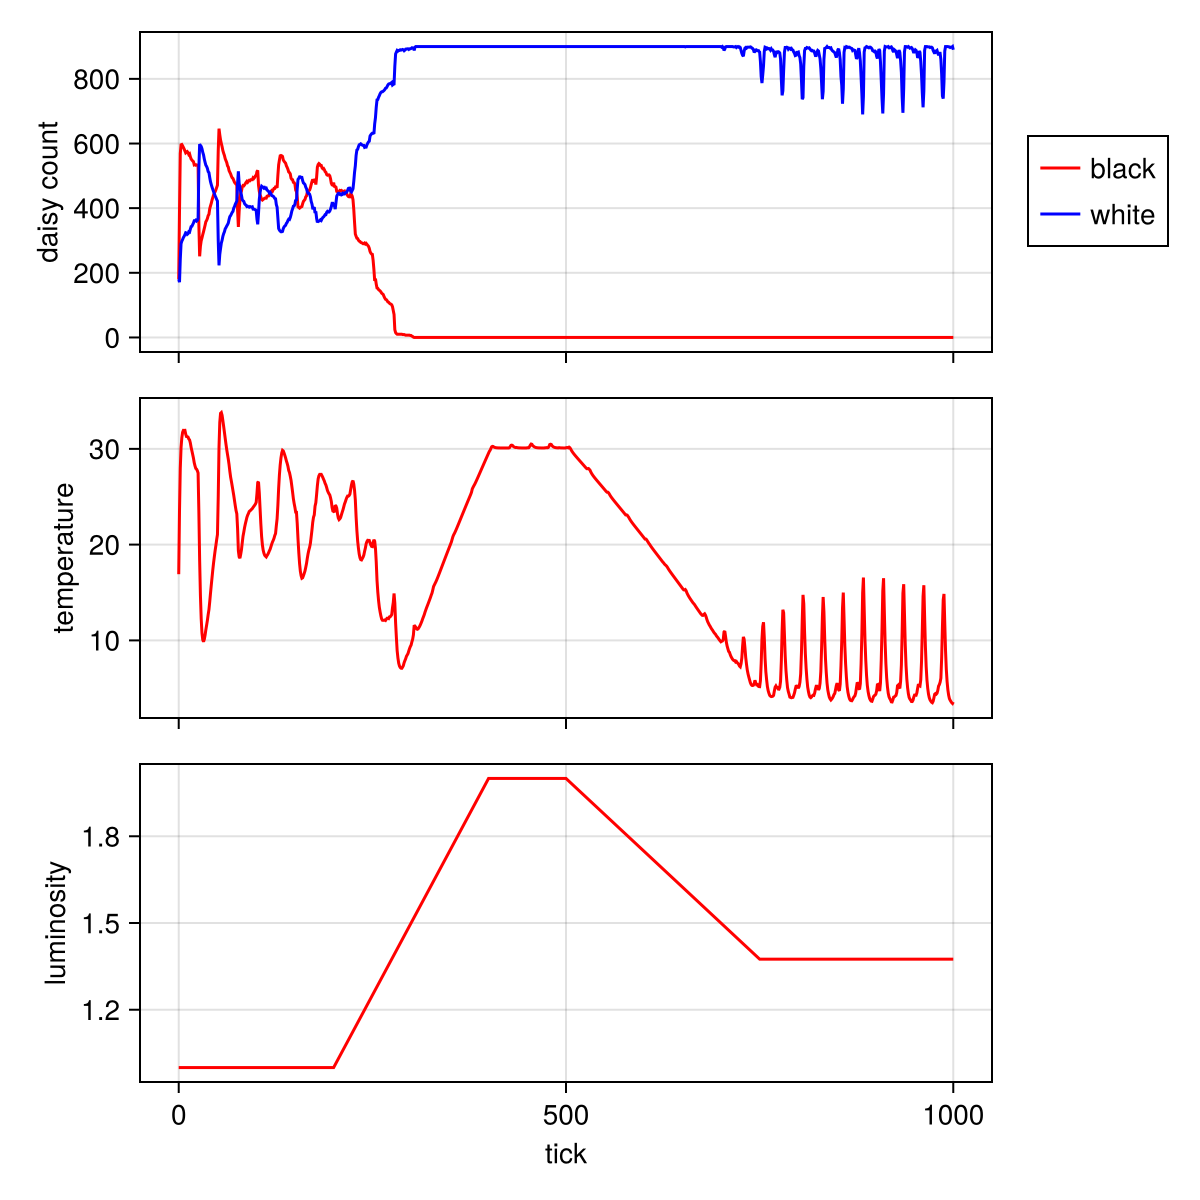
\includegraphics[width=1\linewidth,height=\textheight,keepaspectratio]{image/70.png}
&
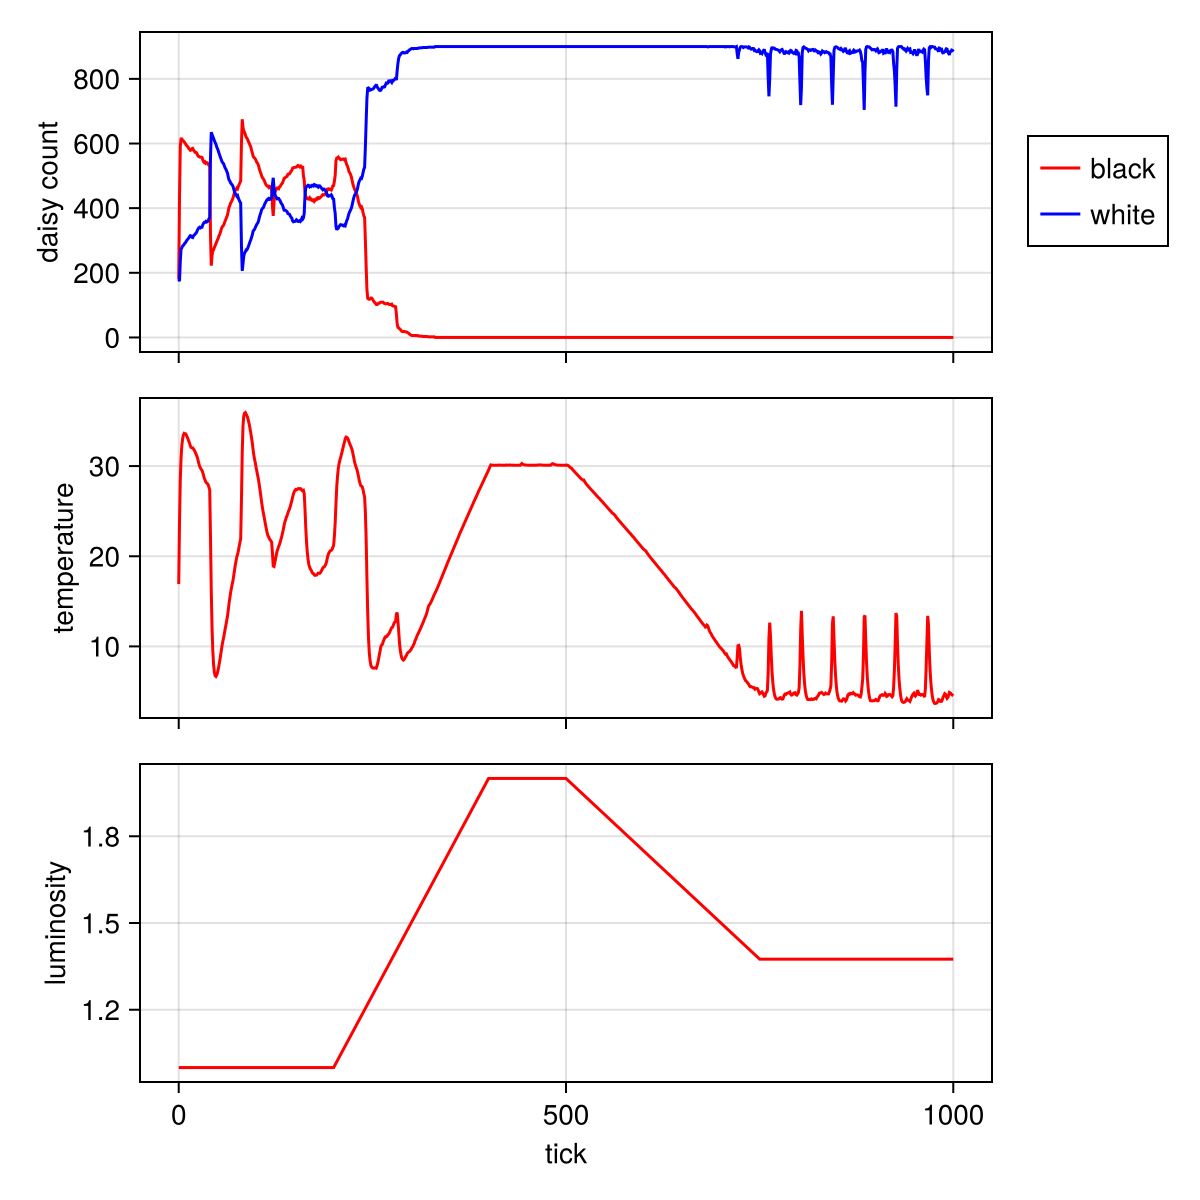
\includegraphics[width=1\linewidth,height=\textheight,keepaspectratio]{image/71.png} \\
Черные доминируют, затем белые & Плавный переход между видами \\
\end{longtable}

\subsection{Комплексные
графики}\label{ux43aux43eux43cux43fux43bux435ux43aux441ux43dux44bux435-ux433ux440ux430ux444ux438ux43aux438-1}

\begin{longtable}[]{@{}cc@{}}
\toprule\noalign{}
max\_age=25, init\_white=0.8 & max\_age=40, init\_white=0.8 \\
\midrule\noalign{}
\endhead
\bottomrule\noalign{}
\endlastfoot
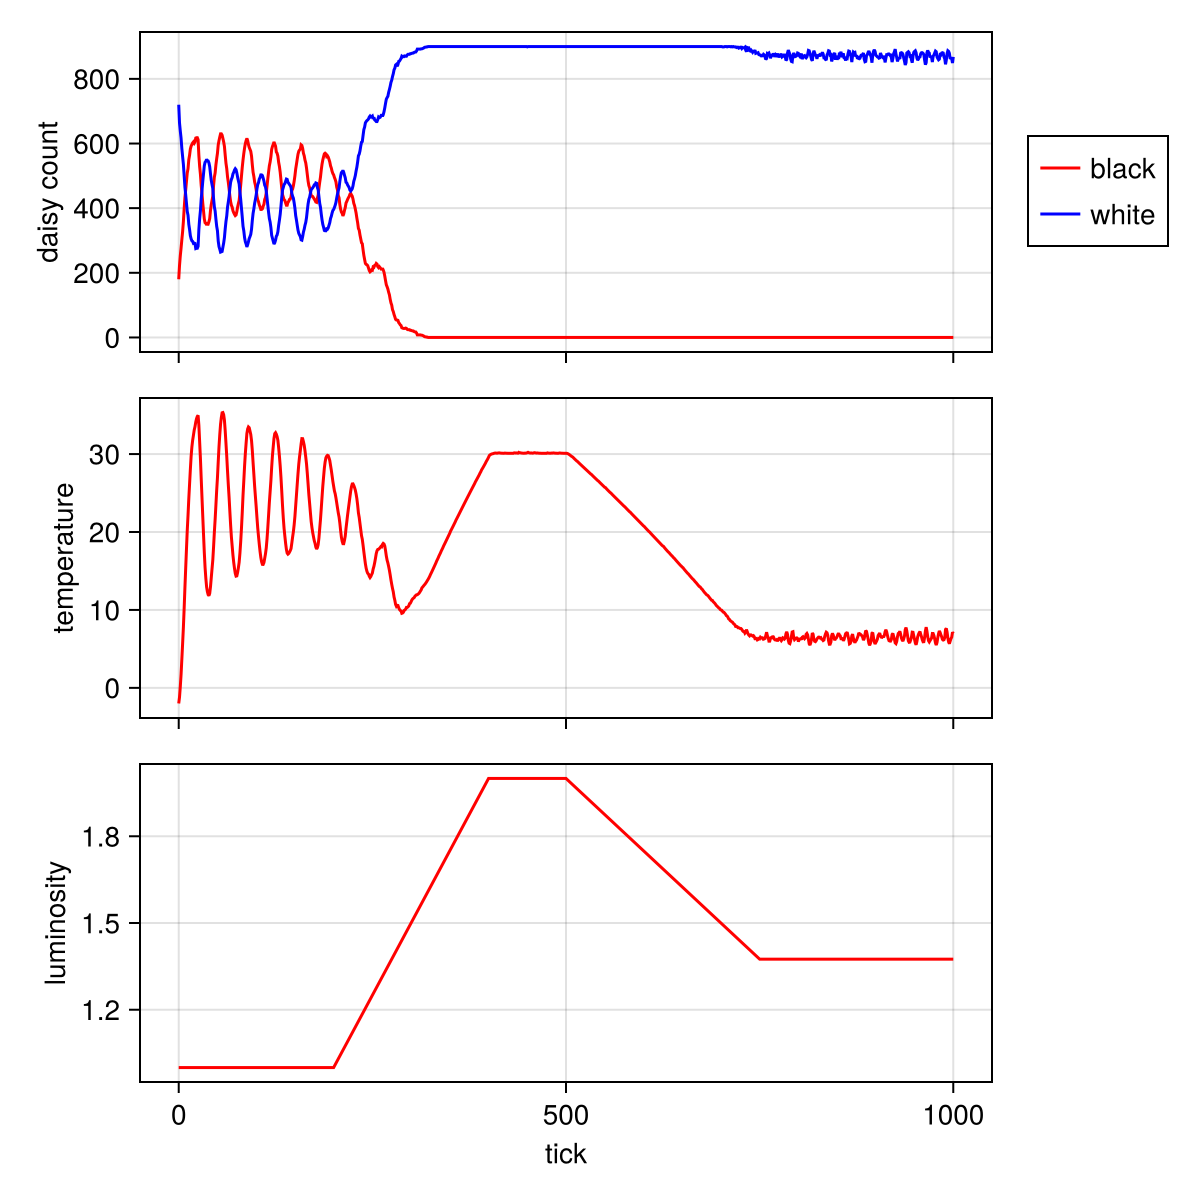
\includegraphics[width=1\linewidth,height=\textheight,keepaspectratio]{image/72.png}
&
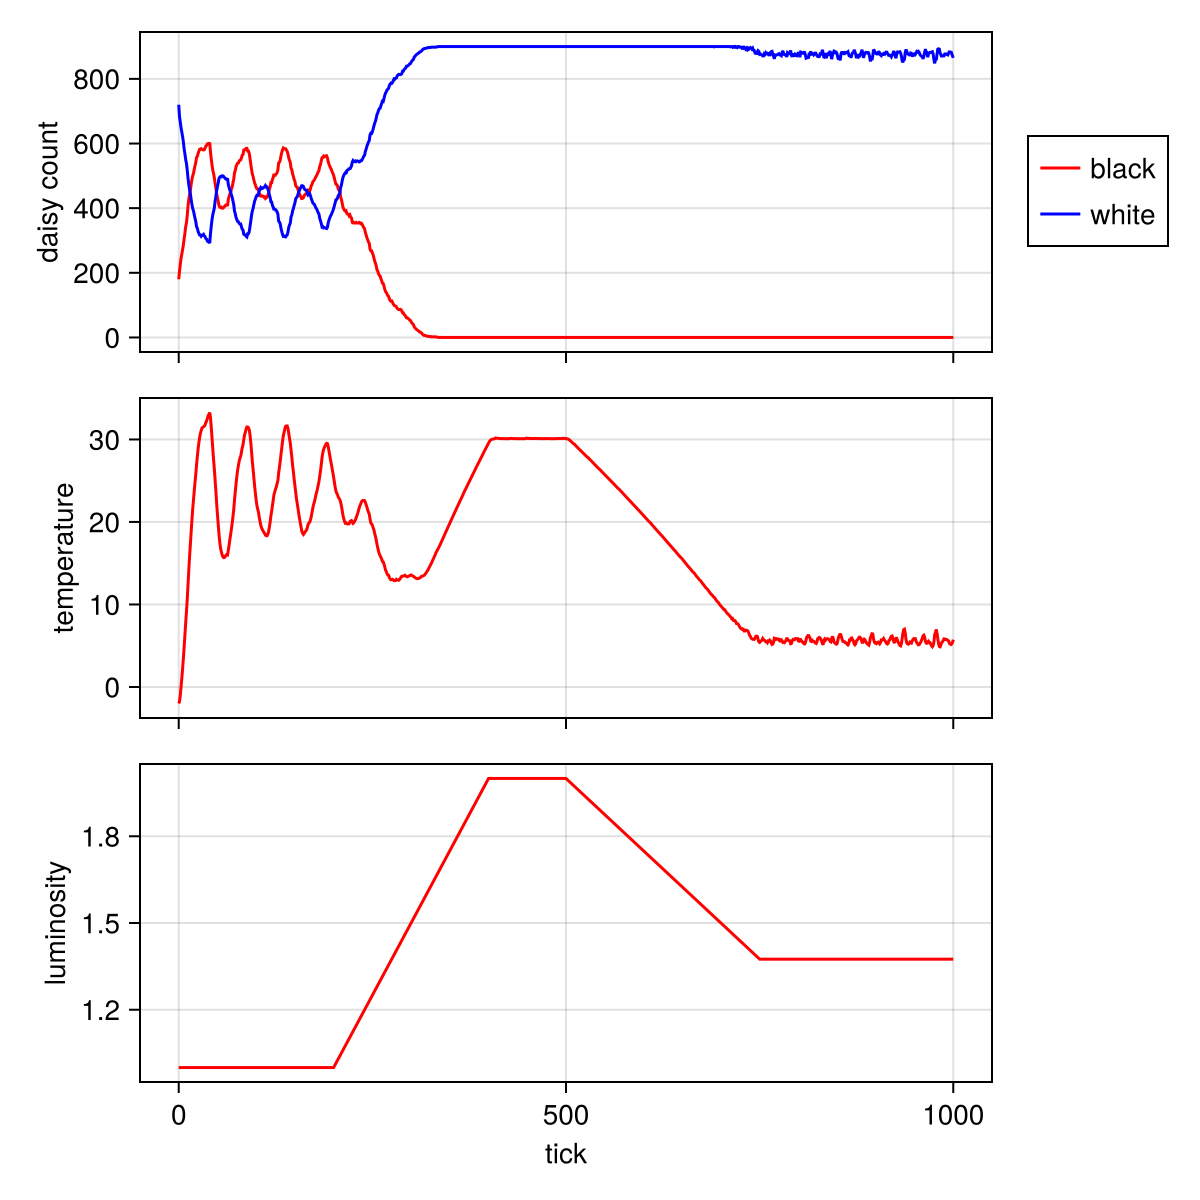
\includegraphics[width=1\linewidth,height=\textheight,keepaspectratio]{image/73.png} \\
Черные доминируют с начала & \textbf{Наилучшая стабилизация
температуры} \\
\end{longtable}

\section{Сводная таблица
результатов}\label{ux441ux432ux43eux434ux43dux430ux44f-ux442ux430ux431ux43bux438ux446ux430-ux440ux435ux437ux443ux43bux44cux442ux430ux442ux43eux432}

\subsection{Влияние параметров на
динамику}\label{ux432ux43bux438ux44fux43dux438ux435-ux43fux430ux440ux430ux43cux435ux442ux440ux43eux432-ux43dux430-ux434ux438ux43dux430ux43cux438ux43aux443}

\begin{longtable}[]{@{}
  >{\raggedright\arraybackslash}p{(\linewidth - 6\tabcolsep) * \real{0.1264}}
  >{\raggedright\arraybackslash}p{(\linewidth - 6\tabcolsep) * \real{0.3563}}
  >{\raggedright\arraybackslash}p{(\linewidth - 6\tabcolsep) * \real{0.2414}}
  >{\raggedright\arraybackslash}p{(\linewidth - 6\tabcolsep) * \real{0.2759}}@{}}
\toprule\noalign{}
\begin{minipage}[b]{\linewidth}\raggedright
Параметры
\end{minipage} & \begin{minipage}[b]{\linewidth}\raggedright
Пространственное распределение
\end{minipage} & \begin{minipage}[b]{\linewidth}\raggedright
Динамика численности
\end{minipage} & \begin{minipage}[b]{\linewidth}\raggedright
Стабилизация температуры
\end{minipage} \\
\midrule\noalign{}
\endhead
\bottomrule\noalign{}
\endlastfoot
max\_age=25, init\_white=0.2 & Преобладание черных & Черные доминируют &
Средняя \\
max\_age=40, init\_white=0.2 & Больше белых & Сильные колебания &
Хорошая \\
max\_age=25, init\_white=0.8 & Белые → черные & Преобладание черных &
Средняя \\
max\_age=40, init\_white=0.8 & Преобладание черных & Плавные колебания &
\textbf{Наилучшая} \\
\end{longtable}

\section{Заключение}\label{ux437ux430ux43aux43bux44eux447ux435ux43dux438ux435}

\subsection{Выводы}\label{ux432ux44bux432ux43eux434ux44b}

\begin{enumerate}
\def\labelenumi{\arabic{enumi}.}
\item
  \textbf{Модель успешно реализована} на Julia с использованием пакетов
  Agents, DrWatson, CairoMakie
\item
  \textbf{Механизм обратной связи} продемонстрирован:

  \begin{itemize}
  \tightlist
  \item
    При повышении светимости увеличивается доля белых маргариток
  \item
    При понижении светимости увеличивается доля черных маргариток
  \item
    Температура остается стабильной
  \end{itemize}
\item
  \textbf{Параметрический анализ} показал:

  \begin{itemize}
  \tightlist
  \item
    Увеличение max\_age → более плавная динамика, лучшая стабилизация
  \item
    Изменение init\_white влияет на начальный этап, но равновесие
    достигается
  \end{itemize}
\item
  \textbf{Наилучший результат} стабилизации температуры:

  \begin{itemize}
  \tightlist
  \item
    \textbf{max\_age = 40, init\_white = 0.8}
  \end{itemize}
\end{enumerate}

\section{Выводы}\label{ux432ux44bux432ux43eux434ux44b-1}

\subsection{Итоги}\label{ux438ux442ux43eux433ux438}

\begin{itemize}
\tightlist
\item
  Освоен агентный подход к имитационному моделированию
\item
  Создана и проанализирована модель Daisyworld
\item
  Выполнена визуализация: анимация, графики, тепловые карты
\item
  Проведено параметрическое исследование
\item
  Освоено литературное программирование с Literate.jl
\item
  Сгенерированы чистый код, Jupyter Notebook, Quarto-документы
\end{itemize}

\textbf{Гипотеза Геи подтверждена:} биота способна регулировать климат в
широком диапазоне внешних условий.

\section{Список
литературы}\label{ux441ux43fux438ux441ux43eux43a-ux43bux438ux442ux435ux440ux430ux442ux443ux440ux44b}

\phantomsection\label{refs}
\begin{CSLReferences}{0}{1}
\end{CSLReferences}




\end{document}
